
\documentclass[11pt]{article}

\usepackage{graphicx}
\usepackage{hyperref}
\usepackage{float}

\begin{document}

    \title{Darstellung von Geometrie in elliptischem Raum}
    \author{Jost Triller}
    \date{12.02.2020}
    \maketitle

    Ziel dieses Projektes ist, 3D-Modelle in der dreidimensionalen Oberfläche einer Hyperkugel aus der Sicht einer
    perspektivischen Kamera in Echtzeit darzustellen.

    Dafür werden werden, statt wie in einem euklidischem Raum dreidimensionale Vektoren, vierdimensionale Einheitsvektoren
    als Positionskoordinaten benutzt.
    Die Rotation dieses Einheitsvektors stellt dabei die Translation von Objekten dar.
    Die Orientation eines Objektes in diesem Raum wird durch drei orthogonale vierdimensionale Vektoren, die für die
    oben-, links-, geradeaus-Richtungen aus der Sicht des Objektes stehen.
    Dabei ist zu beachten, dass diese drei Orientations-Vektoren orthogonal zu der Koordinate (auf der Hyperkugel) sind
    und bei Translation eines Objektes dementsprechend mit rotiert werden müssen.

    \begin{figure}[H]
        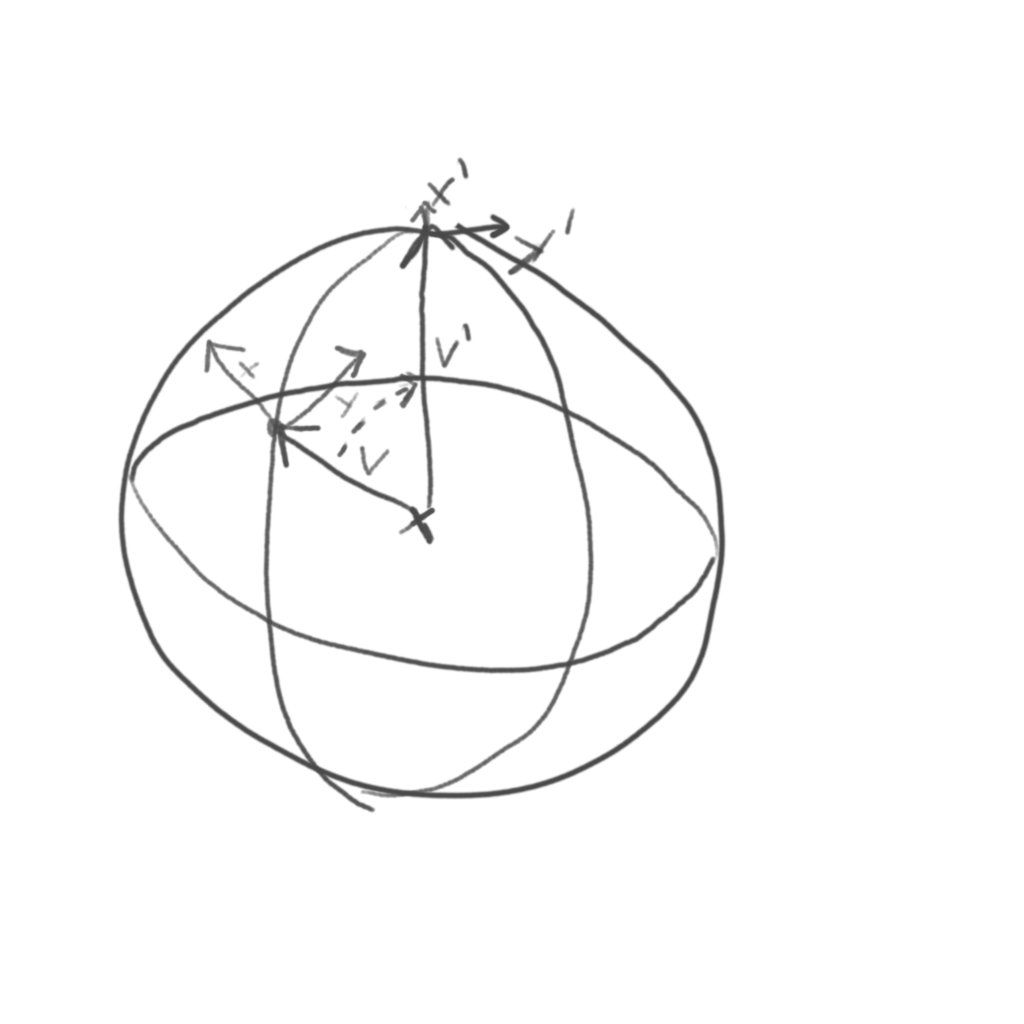
\includegraphics[width=0.8\linewidth]{hypersphere2d.png}
        \caption{Darstellung des Prinzips an einer Kugel. $v$ ist der Koordinatenvektor,
            $x,y$ sind die Orientationsvektoren des Objekts. $v',x',y'$ entsprechen diesen Vektoren nach einer Bewegung}
        \label{fig:hypesphere2d}
    \end{figure}

    Mithilfe dieser Eigenschaften eines Objektes lassen sich nun die Vertices eines 3D-Meshes auf die Oberfläche der Hyperkugel
    projizieren.

    Um die Screenspace-Koordinaten zu bekommen muss jetzt noch der Winkel der Richtung zu einem Punkt relativ zu der
    Sehrichtung der Kamera berechnet werden.
    Dazu wird zunächst die lokale Richtung von der Kamera zu dem gewünschten Punkt berechnet.

    \begin{figure}[H]
        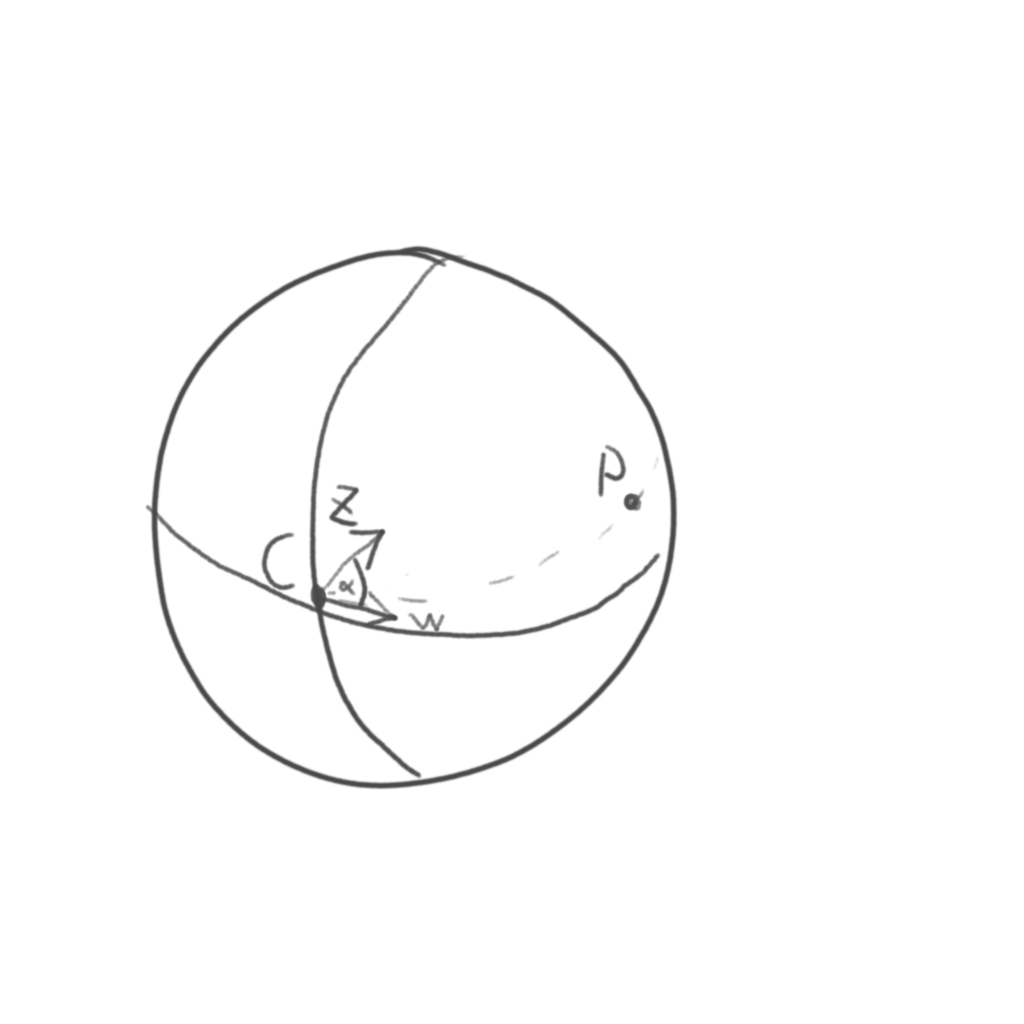
\includegraphics[width=0.8\linewidth]{localDirectionalVektor.png}
        \caption{Die Kamera $C$ schaut in Richtung $z$. Der Punkt $P$ liegt für die Kamera lokal in Richtung $w$.
        $\alpha$ ist der Winkel aus dem abhängig von dem Field-Of-View die Screenspace-Koordinate berechnet wird.}
        \label{fig:localDirectionalVektor}
    \end{figure}

    In der praktischen Umsetzung sind vor allem zwei Effekte auffällig anders zu klassischem Rendering in euklidischem Raum.

    Man kann gerade sich in eine Richtung bewegen und kommt nach einer Weile wieder am Ausgangspunkt an.
    Das ist intuitiv einleuchtend;
    man bewegt sich auf dem einem Großkreis der Hyperkugel ähnlich wie bei einer Reise um die Welt entlang des
    Äquators.

    Zweitens werden sich entfernende Objekte ab einer gewissen Entfernung scheinbar wieder größer und werden ab einem bestimmten
    Punkt vertikal und horizontal gespiegelt dargestellt.
    Warum das so ist, wird mithilfe dieser Graphik klar:

    \begin{figure}[H]
        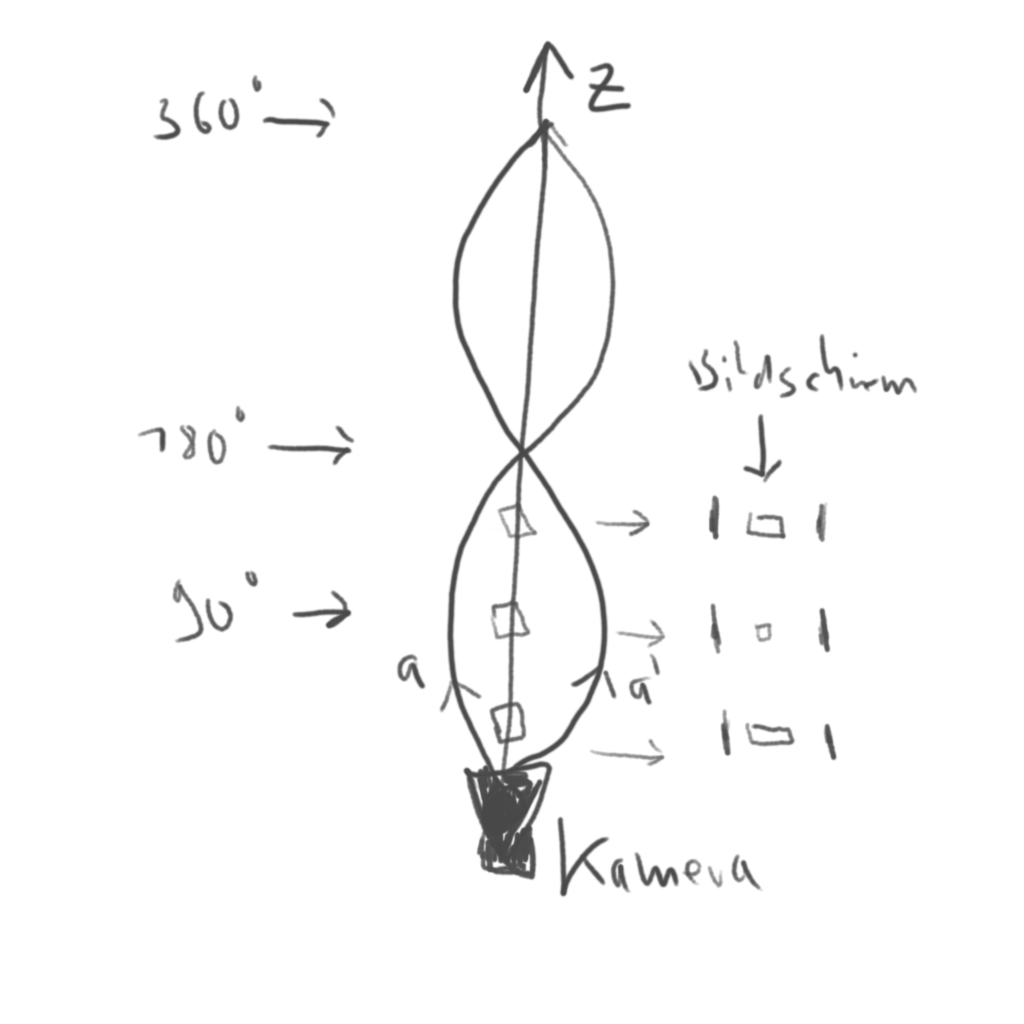
\includegraphics[width=0.8\linewidth]{cameraPerspective.png}
        \caption{
            $z$ ist die Blickrichtung und $a,a'$ sind die beiden das Sichtfeld der Kamera begrenzenden Strahlen.
            Ein Objekt, dass weiter entfernt ist scheint mehr Platz im Sichtfeld einzunehmen als ein gleich großes
            näheres Objekt bei 90 deg.
        }
        \label{fig:cameraPerspective}
    \end{figure}


    \begin{figure}[H]
        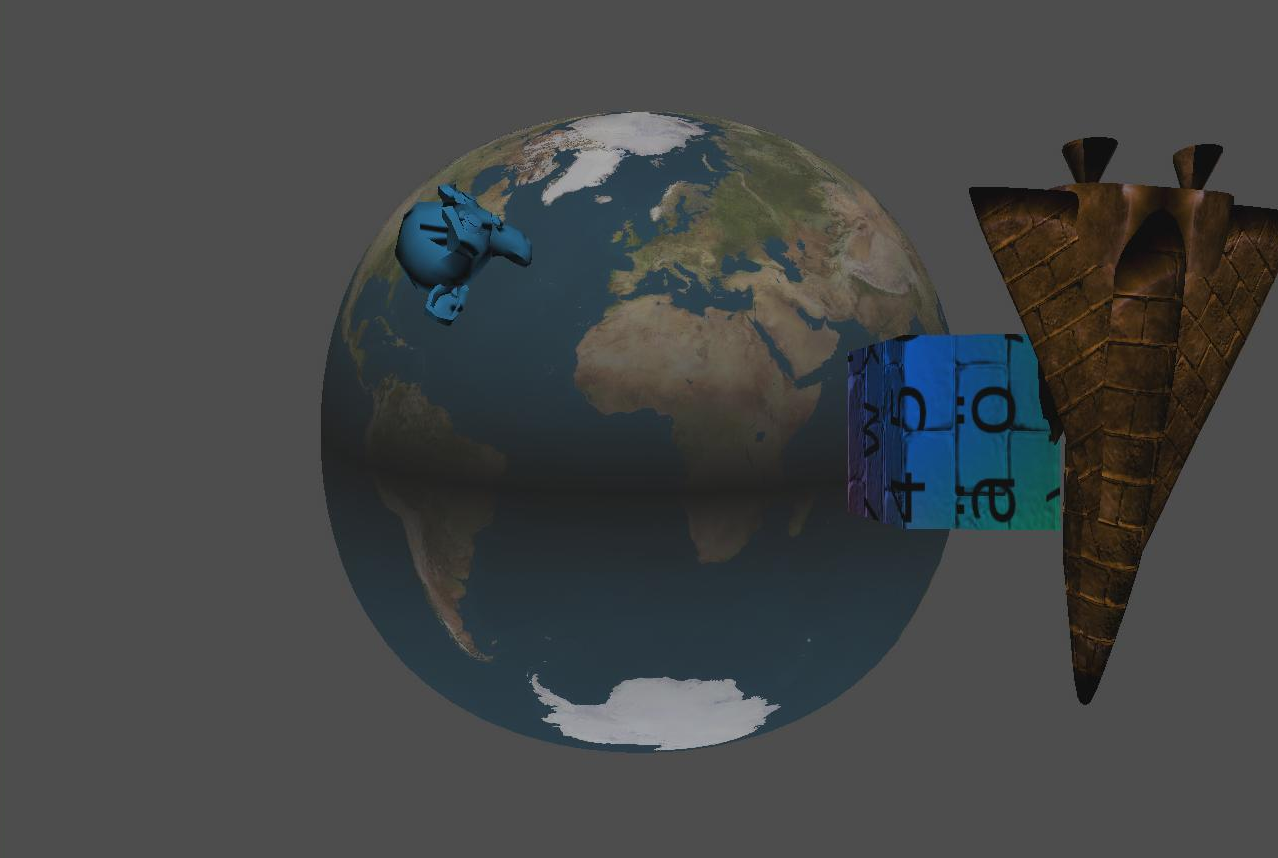
\includegraphics[width=0.8\linewidth]{screenshot.png}
        \caption{
        }
        \label{fig:screenshot}
    \end{figure}

    Der blaue Affenkopf ist als Modell ähnlich groß wie das Modell der Erde.
    Im euklidischen Raum würde man aufgrund der Größenverhältnisse annehmen, dass das Modell der Erde näher
    an der Kamera ist als der blaue Affenkopf. Hier allerdings ist der Affenkopf näher an der Kamera positioniert, was
    man gut daran erkennen kann, dass die Erde den Affenkopf nicht verdeckt.

    Auch zu beachten ist, dass, obwohl es nur eine Punklichtquelle gibt, die Erde augenscheinlich von zwei Seiten beleuchtet
    wird, was allerdings darauf zurückzuführen ist, dass die Erde das Licht der Lichtquelle von beiden Seiten des Großkreises
    erreicht.


    \subsection*{Mittel}

    Benutzt wurde Matlabs symbolische Mathematik-Toolbox um Gleichungssysteme zu lösen, die z.B. die Berechnung eines
    cross-Produktes für vier Dimensionen oder die Berechnung einer zu zwei 4D-Vektoren orthogonalen Ebene beschreiben.

    OpenGL wurde als Graphikbibliothek benutzt, dazu ergänzend glfw \url{https://www.glfw.org/}, GLM
    \url{https://glm.g-truc.net/0.9.9/index.html}, GLI \url{http://gli.g-truc.net/0.8.2/index.html},
    shader-printf \url{https://github.com/msqrt/shader-printf}.

    Zum Laden von Konfigurationen wird nlohmann/json \url{https://github.com/nlohmann/json} benutzt.

    Denkhilfsmittel waren unter anderem Wikipedia für z.B. die Berechnung der 4D-Rotation in einer Ebene,
    learnopengl.com \url{https://learnopengl.com/} für OpenGL Prinzipien, stackoverflow, cppreference und das OpenGL Forum für
    allgemeine C++/OpenGL Programmierprobleme.




\end{document}
